% !TeX document-id = {a04d4f31-1b22-4ab2-a3f9-07505c808c5f}
% !TeX TXS-program:compile = txs:///pdflatex/[--shell-escape]
%% !TeX program = lualatex
\documentclass{article}
\usepackage[paperwidth = 100mm, 
paperheight =47mm, 
textwidth = 100mm,
textheight = 47mm,
nohead,
nofoot,
nomarginpar]{geometry}
\usepackage{amsmath,amsfonts,amssymb}
\usepackage{tikz,pgfplots}
\usetikzlibrary{arrows,arrows.meta,bending,calc,decorations,shadings,shadows,shapes,shapes.arrows,shapes.geometric}
\usetikzlibrary{calc,fadings,decorations.pathreplacing}
\usepgfplotslibrary{units,fillbetween,groupplots,colorbrewer}
\usetikzlibrary{pgfplots.colorbrewer,}
\usepackage{pgfplotstable}
\usetikzlibrary{3d,spy}
\usepgfmodule{plot}
\usepackage{scalerel}
\usepackage{epstopdf}
\newcommand*{\xMin}{-2}%
\newcommand*{\xMax}{9}%
\newcommand*{\yMin}{-4}%
\newcommand*{\yMax}{6.5}%

\definecolor{As}{RGB}{255,255,0}
\definecolor{Al}{RGB}{173,216,230}
\definecolor{Ga}{RGB}{0,128,150}
\begin{document}
	\thispagestyle{empty}
\begin{tikzpicture}[remember picture,overlay]
		%	\draw[step=.5cm,gray,very thin,opacity=0.2] (0,0) grid (\xMax,\yMax);
		%		\foreach \i in {\xMin,...,\xMax} {
			%				\draw [very thin,gray,opacity=0.2] (\i,\yMin) -- (\i,\yMax)  node [below,opacity=1] at (\i,\yMin) {$\i$};
			%													}
		%			\foreach \i in {\yMin,...,\yMax} {
			%					\draw [very thin,gray,opacity=0.2] (\xMin,\i) -- (\xMax,\i) node [left,opacity=1] at (\xMin,\i) {$\i$};
			%						}
		%				
\begin{scope}
	
	
\node[anchor=north,xshift=-15mm] at (current page.north) {Real space};
\node[anchor=north,xshift=25mm] at (current page.north) {$\boldsymbol{k}$-space};
	
\node[anchor=south west,inner sep=0mm,yshift=0mm,opacity=0] (s1) at (current page.south west) {\includegraphics[width=0.5\textwidth]{/media/labfiles/ruco/phd-ssp/phd-codes/structures/GaAs1.pdf}};
\node[anchor=south east,inner sep=0mm,yshift=-3mm,opacity=1] (s2) at (current page.south east) {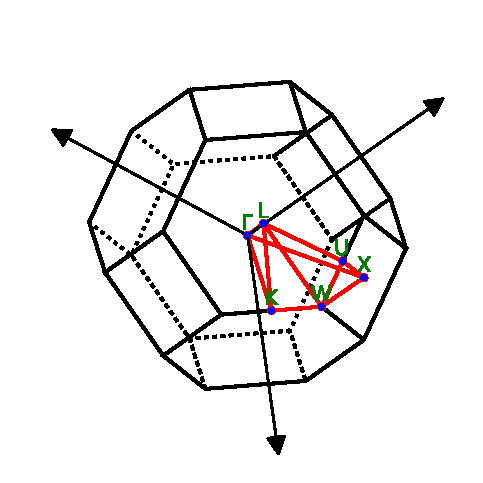
\includegraphics[width=0.5\textwidth]{/media/labfiles/ruco/phd-ssp/phd-codes/atom-structures/01.FCC.pdf}};




\draw[line width=0.2mm,rounded corners=.1mm,densely dashed] 
([xshift=12.5mm,yshift=10.2mm]s1.south west)--
([xshift=18.5mm,yshift=5mm]s1.west)--
([xshift=9mm,yshift=8mm]s1.center)--
([xshift=5mm,yshift=14mm]s1.south)--cycle;
%

%
\draw[line width=0.2mm,rounded corners=.1mm,densely dashed] 
([xshift=5mm,yshift=-5mm]s1.north)--
([xshift=-0.5mm,yshift=-2.5mm]s1.center)--
([xshift=-6.5mm,yshift=1mm]s1.east)--
([xshift=-3mm,yshift=-3.5mm]s1.north east);


\draw[line width=0.2mm,rounded corners=.1mm,densely dashed] 
([xshift=12.5mm,yshift=10.2mm]s1.south west)--
([xshift=-0.5mm,yshift=-2.5mm]s1.center)--
([xshift=-6.5mm,yshift=1mm]s1.east)--
([xshift=5mm,yshift=14mm]s1.south);


\node[anchor=south west,inner sep=0mm,yshift=0mm,opacity=1] (s1) at (current page.south west) {\includegraphics[width=0.5\textwidth]{/media/labfiles/ruco/phd-ssp/phd-codes/structures/GaAs1.pdf}};
%

\draw[line width=0.2mm,rounded corners=.1mm,densely dashed] 
([xshift=18.5mm,yshift=5mm]s1.west)--
([xshift=5mm,yshift=-5mm]s1.north)--
([xshift=-3mm,yshift=-3.5mm]s1.north east)--
([xshift=9mm,yshift=8mm]s1.center);


\shade [ball color=Ga] ([xshift=2mm,yshift=7mm]s1.west) circle (0.2) node[label=right:{Ga}] { } ;
%\shade [ball color=Al] (-3.3,6.5) circle (0.3) node[label=right:{\Large\, Al}] { } ;
\shade [ball color=As] ([xshift=2mm,yshift=1mm]s1.west) circle (0.2) node[label=right:{As}] { };	
\node[anchor=north west, fill=blue, text=white,inner sep=0.5mm,font=\bf] at (current page.north west) {(a)};  
\node[anchor=north east, fill=blue, text=white,inner sep=0.5mm,font=\bf] at (current page.north east) {(b)};   

\end{scope}	

		
		
	\end{tikzpicture}
	
	
\end{document}